\documentclass[12pt]{article}
\usepackage{amsmath,amsfonts,amsthm,fullpage,amssymb}
\usepackage{algorithm}
\usepackage{algorithmic}
\usepackage{graphicx}
\usepackage{url}
\usepackage{titling}
\usepackage[backend=biber,sorting=ynt]{biblatex}
\usepackage{tcolorbox}
\usepackage[colorlinks=true, hidelinks]{hyperref}
\hypersetup{
    colorlinks=true,
    linkcolor=blue,
    citecolor=blue,
}
\usepackage{listings}
\usepackage{xcolor}
\lstdefinestyle{mystyle}{
    backgroundcolor=\color{backcolour},   
    commentstyle=\color{codegreen},
    keywordstyle=\color{magenta},
    numberstyle=\tiny\color{codegray},
    stringstyle=\color{codepurple},
    basicstyle=\ttfamily\footnotesize,
    breakatwhitespace=false,         
    breaklines=true,                 
    captionpos=b,                    
    keepspaces=true,                 
    numbers=left,                    
    numbersep=5pt,                  
    showspaces=false,                
    showstringspaces=false,
    showtabs=false,                  
    tabsize=2
} 
\addbibresource{references.bib}
\setlength{\droptitle}{-3cm} % Moves the title up


\begin{document}

\title{ISYE 6740, Fall 2025, Prof. Yao Xie\\ Homework 4\\{\small 100 points}}
\author{Student Name Here}
\date{}
\maketitle

\vspace{-1cm}
\textbf{Provided Data and Submission Requirements:}
\begin{itemize}
    \item All results, explanations, and math must be included in your PDF submission. Handwritten work is not accepted per the syllabus. Screenshots of work is also not accepted.
    \item If applicable, questions marked with \textbf{GS} must be submitted to Gradescope. Failure to pass gradescope tests will result in penalties to the points for that question.
\end{itemize}

\textbf{This assignment does not have any gradescope requirements}

\textbf{Assignment Data:}
\begin{itemize}
    \item Q4: Comparing Classifiers: Divorce Classification / Prediction [marriage.csv]
\end{itemize}

\subsection*{1. Optimization (25 points).}

Consider a simplified logistic regression problem. 
Given $m$ training samples $(x^i, y^i)$, $i = 1, \ldots, m$. The data $x^i \in \mathbb R$, and $y^i \in \{0, 1\}$.  To fit a logistic regression model for classification, we solve the following optimization problem, where $\theta \in \mathbb R$ is a parameter we aim to find:
\begin{equation}
\max_\theta \ell (\theta), \label{eqn}
\end{equation}
where the log-likelhood function \[\ell(\theta) = \sum_{i=1}^m \left\{-\log (1+\exp\{-\theta^T x^i\}) + (y^i-1) \theta^T x^i\right\}.\]

\begin{enumerate}
\item (5 points) Show step-by-step mathematical derivation for the gradient of the cost function $\ell(\theta)$ in (\ref{eqn}).

{\bf 1.1 Answer:}
\begin{align*}
    \nabla_\theta \ell(\theta) &= \sum_{i=1}^m\nabla_\theta \ell_i(\theta) \\
    \intertext{Take the gradient of individual term. Answer given in the lecture slides} \\
    \frac {\partial \ell^i}{\partial \theta}  &= \frac{e^{-\theta^T x^i}x^i}{1+e^{-\theta^T x^i}} + (y^i -1)x^i \\
\end{align*}

We can see from the lecture slides that the term $\frac{e^{-\theta^T x^i}x^i}{1+e^{-\theta^T x^i}}$ is the term for $p(y=0|x,\theta)$, so we can also take this as $(1-p(y=1|x,\theta))$. In the notes, $p(y=1|x,\theta) = \sigma(\theta^Tx)$. So we can substitute the sigmoid function into the gradient:

\begin{align*}
    \frac {\partial \ell^i}{\partial \theta}  &= (1-\sigma(\theta^T x^i))x^i + (y^i -1)x^i \\
    \frac {\partial \ell^i}{\partial \theta}  &= (y^i -\sigma(\theta^T x^i))x^i \\
\end{align*}

So, the gradient is this equation applied to all $i$:
\begin{align*}
    \nabla_\theta \ell(\theta) &= \sum_{i=1}^m(y^i -\sigma(\theta^T x^i))x^i \\
\end{align*}

\item (5 points) Write a pseudo-code  for performing {\bf gradient descent} to find the optimizer $\theta^*$. This is essentially what the training procedure does.

{\bf 1.2 Answer:}

\begin{lstlisting}
Initialize Theta and set max iterations
Loop until max iterations or convergence:
    old_gradient = gradient # save previously calculated gradient
    
    # calculate gradient of all samples:
    gradient = sum(x[i](y[i] 
        - sigmoid(theta.T * x[i])) for i in range(m))

    # update theta:
    theta = theta + learning_rate * gradient

    # check convergence:
    if gradient - old_gradient < tolerance:
        break
return theta
\end{lstlisting}

\item (5 points) Write the pseudo-code for performing the {\bf stochastic gradient descent} algorithm to solve the training of logistic regression problem (\ref{eqn}). Please explain the difference between gradient descent and stochastic gradient descent for training logistic regression.

{\bf 1.3 Answer:} This is largely the same as the previous answer, but it randomly selects individual samples to perform the gradient calculation and theta update instead of calculating on all samples. This makes it more efficient for large datasets, but also more noisy.

\begin{lstlisting}
initialize theta and set max iterations
loop until max iterations or convergence:
    old_gradient = gradient # save previously calculated gradient
    
    subset_x, subset_y = random_sample(data, step_size)

    # calculate gradient of subset samples:
    gradient = sum(subset_x[i](subset_y[i] 
            - sigmoid(theta.T * subset_x[i])) for i in range(step_size))

    # update theta:
    theta = theta + learning_rate * gradient

    # check convergence by seeing if likelihood is close to zero:
    if ||gradient|| < tolerance:
        break
return theta
\end{lstlisting}

\item (10 points) We will {\bf prove that the training problem in basic logistic regression problem is concave.} Derive the Hessian matrix of $\ell(\theta)$ and based on this, show the training problem (\ref{eqn}) is concave. Explain why the problem can be solved efficiently and gradient descent will achieve a unique global optimizer, as we discussed in class. 
\end{enumerate}

{\bf 1.4 Answer:} The Hessian is the second derivative of the function. We can arrive there by taking the derivative of the gradient w.r.t $\theta$ again.

\begin{align*}
    \nabla_\theta^2 \ell(\theta) &= \sum_{i=1}^m(\frac {\partial} {\partial \theta}(y^i -\sigma(\theta^T x^i))x^i) \\
    \intertext{Derivative of sigmoid \cite{se1225116}:}\\
    \frac{\partial}{\partial x} \sigma(x) &= \sigma(x)(1-\sigma(x)) \\
    \intertext{And derive the internal sigmoid term for chain rule:}\\
    \frac {\partial \theta^T x^i} \partial {\theta} &= x^i
    \intertext{Apply sigmoid derivation and chain rule:} \\
    \nabla_\theta^2 \ell(\theta) &= \sum_{i=1}^m(-\sigma(\theta^T x^i)(1-\sigma(\theta^T x^i))x^i(x^i)^{T})
\end{align*}

To prove concave, we can multiply the Hessian by a vector and analyze if the result is negative: $z^T H z \leq 0$ \cite{se1225116}.
\begin{align*}
    z^T H z &= z^T (-\sum_{i=1}^m(\sigma(\theta^T x^i)(1-\sigma(\theta^T x^i))x^i(x^i)^{T})) z \\
    &= -\sum_{i=1}^m(\sigma(\theta^T x^i)(1-\sigma(\theta^T x^i)))(z^T x^i(x^i)^{T} z) \\
    &= -\sum_{i=1}^m(\sigma(\theta^T x^i)(1-\sigma(\theta^T x^i)))(z^T x^i)^2
\end{align*}
The following terms in the Hessian cannot be negative:
\begin{align*}
    \sigma(\theta^T x^i)& \quad\text{This is a probability, so between [0,1]}\\
    1-\sigma(\theta^T x^i)& \quad\text{Also [0,1] due to above}\\
    (z^T x^i)^2& \quad\text{Squared term must be $\geq 0$}
\end{align*}

Since all the terms are non-negative, the negative sign in front of the summation means $z^T H z \leq 0$. This means the Hessian is negative semi-definite, which means the function is concave.

\subsection*{2. {\it Fair} Gaussian mixture model (25 points).}

This question builds on EM for GMM model estimation, as well as optimization lectures; the purpose is to practice constrained optimization. 
Recall the EM step in the estimation of Gaussian mixture models. Now suppose that in addition to all the original setup, we require a {\it fairness} constraint: the weights of the Gaussian components cannot be smaller than a pre-specified constant $c$. We will derive a modified EM algorithm for the Gaussian model, with two components $K = 2$, when the weights for each component are required to be greater than $c$: $\pi_1 \geq c$, and $\pi_2 \geq c$ (with $c<0.5$). \\

Show the modified EM algorithm, as well as the complete mathematical derivations. \\

\textit{\small Hint: The only thing you will need to change is that in the M-step, we have to solve a constrained optimization problem with the original constraint $\pi_1+\pi_2 = 1$, as well as $\pi_1 > c$ and $\pi_2 > c$. You will need to introduce additional Lagrangian multipliers for the new constraints and discuss the cases when the constraints are active (or not active) using the KKT condition (in particular, the complementarity condition).}

{\bf Answer:}

Expectation: The expectation step is not modified by the extra constraints.

\[
    \tau_k^i = \frac{\pi_k \mathcal{N}(x^i | \mu_k,\Sigma_k)}{\sum_{k'=1...K}\pi_{k'}\mathcal{N}(x^i | \mu_k,\Sigma_k)}
\]

Maximization: The maximization step incorporates the constraint terms. Without the extra terms, the objective function is:
\[
    f(\theta) = \sum_{i=1}^m \sum_{k=1}^K \tau_k^i(\log(\pi_k) - \frac{1}{2}(x^i-\mu_k)^T \Sigma_k^{-1}(x^i-\mu_k)-\frac{1}{2}\log(|\Sigma_k|)-\frac{n}{2}\log(2\pi))
\]

With the initial constraint Lagrangian term:
\[
    f(\theta) = \sum_{i=1}^m \sum_{k=1}^K \tau_k^i(\log(\pi_k) - \frac{1}{2}(x^i-\mu_k)^T \Sigma_k^{-1}(x^i-\mu_k)-\frac{1}{2}\log(|\Sigma_k|)-\frac{n}{2}\log(2\pi)) + \lambda(1-\sum_{i=1}^K \pi_k)
\]

So, we need to add additional Lagrangian terms to enforce the constraint. I will make these $\lambda_1$ and $\lambda_2$ while designating the initial constraint $\lambda_0$. Additionally, I will expand the $\pi$ summations since $K=2$.
\begin{align*}
    f(\theta) = \sum_{i=1}^m \sum_{k=1}^K \tau_k^i(\log(\pi_k) - \frac{1}{2}(x^i-\mu_k)^T \Sigma_k^{-1}(x^i-\mu_k)-\frac{1}{2}\log(|\Sigma_k|)-\frac{n}{2}\log(2\pi)) \\+ \lambda_0(1 - \pi_1 - \pi_2 ) + \lambda_1(c-\pi_1) + \lambda_2(c-\pi_2)
\end{align*}

As far as the maximization goes, we perform the usual steps: take the partial derivatives and set equal to zero. We can see that the extra constraints didn't impact the $\mu_k$ or $\Sigma_k$ terms, so their values are unchanged from what we already know:
\[
    \mu_k=\frac{\sum_{i=1}^k \tau_k^i x^i}{\sum_{i=1}^k \tau_k^i} \quad
    \Sigma_k=\frac{\sum_{i=1}^k \tau_k^i(x^i-\mu_k)(x^i-\mu_k)^T}{\sum_{i=1}^k \tau_k^i}
\]

The constraints impact the maximization of $\pi_k$. As seen in the normal EM derivation, the terms unrelated to $\pi_k$ drop out. We will take derivatives with respect to $\pi_1$ and $\pi_2$.
\begin{align*}
    0 =\frac{\partial L}{\partial \pi_1} &= \frac{\partial}{\partial \pi_1}\lambda_0(1 - \pi_1 - \pi_2 ) + \lambda_1(c-\pi_1) + \lambda_2(c-\pi_2) + \sum_{i=1}^m (\tau_1^i\log\pi_1)+(\tau_2^i\log\pi_2)\\
    &= -\lambda_0 - \lambda_1 +  \frac{\sum_{i=1}^m \tau_1^i}{\pi_1}\\
    \lambda_0 + \lambda_1  &= \frac{\sum_{i=1}^m \tau_1^i}{\pi_1}\\
    0 =\frac{\partial L}{\partial \pi_2} &= \frac{\partial}{\partial \pi_2}\lambda_0(1 - \pi_1 - \pi_2 ) + \lambda_1(c-\pi_1) + \lambda_2(c-\pi_2) + \sum_{i=1}^m (\tau_1^i\log\pi_1)+(\tau_2^i\log\pi_2) \\
     &= -\lambda_0  - \lambda_2 + \frac{\sum_{i=1}^m \tau_2^i}{\pi_2} \\
     \lambda_0 + \lambda_2 &= \frac{\sum_{i=1}^m \tau_2^i}{\pi_2} \\
\end{align*}

These equations are also the stationary conditions of KKT. We need to show Primal feasibility, dual feasibility, and complementary slackness \cite{enwiki:1310095500}. For a solution to be optimal, it must satisfy all 4 condition categories.

{\textbf Primal feasibility:}
\begin{align*}
\pi_1 + \pi_2 = 1 \\
\pi_1 \geq c \\
\pi_2 \geq c 
\end{align*}

{\textbf Dual feasibility:}
\begin{align*}
\lambda_1 \geq 0 \\
\lambda_2 \geq 0 
\end{align*}

{\textbf Complementary slackness:}
\begin{align*}
\lambda_1(c-\pi_1) = 0 \\
\lambda_2(c-\pi_2) = 0
\end{align*}

Since there are two inequality constraints, there are four cases to consider.

{\bf Neither fairness constraint is active:} 
If neither constraint is active, then $\lambda_1, lambda_2 = 0$, meaning they don't affect the equations. In this case, we can update the $\pi_k$ equations to:
\begin{align*}
    \pi_1 &= \frac{\sum_{i=1}^m \tau_1^i}{\lambda_0} \\
    \pi_2 &= \frac{\sum_{i=1}^m \tau_2^i}{\lambda_0} \\
    \intertext{Substitute this into the original constraint:}\\
    1 &=\frac{\sum_{i=1}^m \tau_1^i}{\lambda_0}+ \frac{\sum_{i=1}^m \tau_2^i}{\lambda_0} \\
    \lambda_0 &= \sum_{i=1}^m \tau_1^i + \sum_{i=1}^m \tau_2^i = m\\
    \intertext{Substituting back into the $\pi_k$ equations:}\\
    \pi_1 &= \frac{\sum_{i=1}^m \tau_1^i}{m} \\
    \pi_2 &= \frac{\sum_{i=1}^m \tau_2^i}{m} \\
\end{align*}

These $\pi$ equations are the same as the normal EM algorithm, which is to be expected since the extra fairness constraints are not active. These are valid if the equations are both $\geq c$, but the next cases explore what happens if that is not true.

{\bf Either constraint is active:}
If $\frac{\sum_{i=1}^m \tau_1^i}{m} \geq c$ does not hold or  $\frac{\sum_{i=1}^m \tau_2^i}{m} \geq c$ does not hold (but not both at the same time), this means that the constraint for one of the $pi$ terms is active. In the case of the active constraint:
\[
\lambda(c-\pi) = 0 \implies \pi = c
\]

And given $\pi_1 + \pi_2 = 1$, the other $pi$ term is $1-c$.

{\bf Both constraints are active:}

This cannot be true. From the same logic in the case above, this would require $\pi_1,pi_2 = c$. This cannot be true because that would require $c=0.5$ to satisfy the original constraint $pi_1 + pi_2 = 1$, which is specifically disallowed in the problem formulation.

{\bf How this impacts the algorithm:}
EM acts as usual until calculating the $\pi_k$ terms. At that point, if the $\pi_k \geq c$, then the normal maximization continues. If that is not the case, then the constraint $\pi_{active} = c$ and $\pi_{inactive} = 1-c$.

\subsection*{3. Bayes Classifier for spam filtering (30 points)} 

In this problem, we will use the  Bayes Classifier algorithm to fit a spam filter by hand. This will enhance your understanding to the Bayes classifier and build intuition. This question does not involve any programming but only derivation and hand calculation. Tools can be used (Python, Excel, Etc.) but all calculations and derivations must still be provided in your report.

Spam filters are used in all email services to classify received emails as ``Spam'' or ``Not Spam''. A simple approach involves maintaining a vocabulary of words that commonly occur in ``Spam'' emails and classifying an email as ``Spam'' if the number of words from the dictionary that are present in the email is over a certain threshold.
We are given the vocabulary consists of 15 words \[V=\{\textsf{free, cheese, pizza, get, fast, now, order, available, slice, offer, not, good, pepperoni, tastes, crust}\}.\] We will use $V_i$ to represent the $i$th word in $V$. Use the training set provided in the table below.

\begin{table}[H]
    \centering
    \begin{tabular}{|c|c|}
        \hline
        \textbf{Spam} & \textbf{Non Spam} \\
        \hline
        \textsf{free cheese pizza get fast now} & \textsf{good pepperoni cheese pizza now available} \\
        \hline
        \textsf{order available pizza slice fast} & \textsf{pepperoni pizza tastes good} \\
        \hline
        \textsf{pizza offer not good} & \textsf{pizza crust tastes not good} \\
        \hline
        & \textsf{cheese slice now pizza} \\
        \hline
    \end{tabular}
    \caption{Spam and Non-Spam Messages}
    \label{tab:sentiment_messages}
\end{table}

Recall that the Naive Bayes classifier assumes the probability of an input depends on its input feature. The feature for each sample is defined as
$x^{(i)} = [x_1^{(i)}, x_2^{(i)}, \ldots, x_d^{(i)}]^T$, $i = 1, \ldots, m$ and the class of the $i$th sample is $y^{(i)}$. In our case the length of the input vector is $d = 15$, which is equal to the number of words in the vocabulary $V$. Each entry $x_j^{(i)}$ is equal to the number of times word $V_j$ occurs in the $i$-th message. 

\begin{enumerate}
\item (5 points) Calculate class prior $\mathbb P(y = 0)$ and $\mathbb P(y = 1)$ from the training data, where $y = 0$ corresponds to spam messages, and $y = 1$ corresponds to non-spam messages. Note that these class prior essentially corresponds to the frequency of each class in the training sample. Write down the feature vectors for each spam and non-spam messages.

{\bf 3.1 Answer:} As mentioned, the priors are just the proportion of the class in the training data:

\[
    P(y=0) = \frac{3}{7} \quad
    P(y=1) = \frac{4}{7}
\]

The feature vectors are a mapping of prevalence from the given message to the word table.
\begin{table}[H]
    \centering
    \begin{tabular}{|c|c|}
        \hline
        \textbf{Spam} & \textbf{Non Spam} \\
        \hline
        \textsf{111111000000000} & \textsf{011001010001100} \\
        \hline
        \textsf{001010111000000} & \textsf{001000000001110} \\
        \hline
        \textsf{001000000111000} & \textsf{001000000011011} \\
        \hline
        & \textsf{011001001000000} \\
        \hline
    \end{tabular}
\end{table}

\item (15 points)  Assuming the keywords follow a multinomial distribution, the likelihood of a sentence with its feature vector $x$ given a class $c$ is given by 
\[
 \mathbb P (x|y = c) = \frac{n!}{x_1! \cdots x_d!}\prod_{k=1}^d \theta_{c, k}^{x_k}, \quad c = \{0, 1\}
\]
where $n = x_1 + \cdots x_d$, $0 \leq \theta_{c,k} \leq 1$ is the probability of word $k$ appearing in class $c$, which satisfies 
\[\sum_{k=1}^d \theta_{c,k} = 1, \quad c = \{0, 1\}.\] Given this, the complete log-likelihood function for our training data is given by
\[
\ell(\theta_{0,1}, \ldots, \theta_{0, d}, \theta_{1,1}, \ldots, \theta_{1, d}) = 
\sum_{i=1}^m \sum_{k=1}^d x_k^{(i)} \log \theta_{y^{(i)}, k}
\]
(In this example, $m = 7$.)
 Calculate the maximum likelihood estimates of $\theta_{0,1}$, $\theta_{0,5}$, $\theta_{1,2}$, $\theta_{1,15}$ by maximizing the log-likelihood function above.\\
 (Hint: We are solving a constrained maximization problem and you will need to introduce Lagrangian multipliers and consider the Lagrangian function.)

{\bf 3.2 Answer: }The constraint $\sum_{k=1}^d \theta_{c,k} = 1, \quad c = \{0, 1\}$ is actually two constraints. Using the bag of words example, this constraint says that "when pulling words from the spam bag, the sum of the probabilities of pulling each word in this class is 1 \supercite{ED_Brent_Speelman}." More simply, within each bag, all the word probabilities in that bag must sum to 1. The two constraints look like:

\[
\sum_{k=1}^d \theta_{0,k} = 1, \sum_{k=1}^d \theta_{1,k} = 1
\]

 To maximize this function, we use the Lagrangian to incorporate the constraints directly into the function. 
 \begin{align*}
    \ell(\theta_{c,k}) &= \sum_{i=1}^m \sum_{k=1}^d x_k^{(i)} \log \theta_{y^{(i)}, k} - \lambda_0(1-\sum_{k=1}^d \theta_{y^i=0,k}) - \lambda_1(1-\sum_{k=1}^d \theta_{y^i=1,k})
 \end{align*}

 The Lagrangian multipliers $\lambda_c$ acts as punishment terms for exceeding the constraints. Since $1-\sum_{k=1}^d \theta_{c,k}$ is distributed to lambda, exceeding the constraints $\sum_{k=1}^d \theta_{c,k}$ results in a negative term in the function. If the parameters exceed the constraints, the Lagrangian multiplier reduces the objective function, and those parameters are unlikely to be the maximized parameters.

From the theory of the bag of words model, we are going to calculate the likelihood of pulling each string of words from the spam bag and the non-spam bag. That's what the likelihood function is calculating. It is easier to understand the function by breaking the generalized form into each class $c=y^i$ to match the constraints. We can split the $\sum_{i=1}^m$ term based on which vectors belong to each class.

\begin{align*}
    \ell(\theta_{0,k}) &= \sum_{i\in c=0}\sum_{k=1}^d x_k^{(i)} \log  \theta_{0, k} - \lambda_0(1-\sum_{k=1}^d \theta_{y^i=0,k}) \\
    \ell(\theta_{1,k}) &= \sum_{i\in c=1}\sum_{k=1}^d x_k^{(i)} \log  \theta_{1, k} - \lambda_1(1-\sum_{k=1}^d \theta_{y^i=1,k})
    \intertext{Generalized:}
    \ell(\theta_{c,k}) &= \sum_{i\in c}\sum_{k=1}^d x_k^{(i)} \log  \theta_{c, k} - \lambda_c(1-\sum_{k=1}^d \theta_{y^i=c,k})
\end{align*}

This function looks the same as the given function, but it splits the summation over all vectors to summation of vectors within each class. This also allows us to split the lagrangian multipliers to each class, meaning we do not have to take both into account with the partial derivatives. We can take the partial derivative set to 0 to solve for any given $\theta_{c,k}$. Since we are only finding one parameter, we can remove the summation over $k$.

\begin{align*}
    \frac{\partial \ell(\theta_{c,k})}{\partial \theta_{c,k}} = 0 &=\frac{\partial}{\partial \theta_{c,k}} \sum_{i\in c} \log  \theta_{c, k} - \lambda_c(1-\theta_{c,k}) \\
    0 &=\frac{\sum_{i\in c} x_k^{(i)}}{\theta_{c,k}} - \lambda_c\\
    \theta_{c,k} &=\frac{\sum_{i\in c} x_k^{(i)}}{\lambda_c}\\
\end{align*}

\begin{align*}
    \frac{\partial \ell(\theta_{c,k})}{\partial \lambda_c} = 0 &=\frac{\partial}{\partial \lambda_c} \sum_{i\in c}\sum_{k=1}^d x_k^{(i)} \log  \theta_{c, k} - \lambda_c(1-\sum_{k=1}^d \theta_{y^i=c,k}) \\
    0 &=\frac{\partial}{\partial \lambda_c}( - \lambda_c + \lambda_c\sum_{k=1}^d \theta_{c,k}) \\
    0 &=( - 1 + \sum_{k=1}^d \theta_{c,k}) \\
    1 &=(\sum_{k=1}^d \theta_{c,k})
\end{align*}

This answer is the same as the constraint. We can substitute our answer for $\theta_{c,k}$ into the constraint to solve for $\lambda_c$.

\begin{align*}
    1 &=(\sum_{k=1}^d \frac{\sum_{i\in c} x_k^{(i)}}{\lambda_c}) \\
    \lambda_c &= \sum_{k=1}^d \sum_{i\in c} x_k^{(i)}
\end{align*}

So, the optimal $\lambda_c$ is the total number of words in class $c$. So, putting this into the earlier equation for $\theta_{c,k}$, we get:

\begin{align*}
    \theta_{c,k} &= \frac{\sum_{i\in c} x_k^{(i)}}{\sum_{k=1}^d \sum_{i\in c} x_k^{(i)}}
\end{align*}

From this equation, we can see that the likelihood of pulling word $k$ from class $c$ is the number of times the word appears in class $c$ divided by the number of words in class $c$, which makes logical sense. We can use this generalized equation to calculate the requested likelihoods.
\begin{align*}
    \theta_{0,1} &= \frac{1}{15}\\
    \theta_{0,5} &= \frac{2}{15}\\
    \theta_{1,2} &= \frac{2}{19}\\
    \theta_{1,15} &= \frac{1}{19}
\end{align*}

\item (10 points) Given a test message ``\textsf{cheese pizza available}``, using the Naive Bayes classifier that you have trained in Part (a)-(b), to calculate the posterior and decide whether it is spam or not spam. Derivations must be shown in your report.

{\bf 3.3 Answer:} The feature vector for this message is: $[011000010000000]$. We will use Bayes Theorem to calculate the posterior probability that the message belongs to spam and non-spam. We will compare these probabilities and choose the higher probability for classification. Bayes Theorem is: 
\[P(C|x) = \frac{P(x|C)P(C)}{P(x)} = \frac{P(x|C)P(C)}{\sum_C P(x|C)P(C)}\]

We already calculated the prior probabilities in 3.1. We will first calculate the per-word likelihoods for each class.
\begin{align*}
\theta_{0,2} &= \frac{1}{15} \\
\theta_{0,3} &= \frac{3}{15} \\
\theta_{0,8} &= \frac{1}{15} \\
\theta_{1,2} &= \frac{2}{19} \\
\theta_{1,3} &= \frac{4}{19} \\
\theta_{1,8} &=\frac{1}{19}
\end{align*}

We can use the given formula to calculate the likelihood of the message for each class.
\[
 \mathbb P (x|y = c) = \frac{n!}{x_1! \cdots x_d!}\prod_{k=1}^d \theta_{c, k}^{x_k}, \quad c = \{0, 1\}
\]

However, we can ignore the $\frac{n!}{x_1! \cdots x_d!}$ term since it is the same for both classes. By that same logic, we can also ignore the $P(X)$ term in Bayes Theorem. So, in the end, we just need to calculate $P(x|C)P(C)$ for each class and compare them.

\begin{align*}
    P(x|C=0) &\propto \theta_{0,2} \times \theta_{0,3} \times \theta_{0,8} =  \frac{1}{15} \times\frac{3}{15} \times \frac{1}{15} \\
    P(x|C=1) &\propto \theta_{1,2} \times \theta_{1,3} \times \theta_{1,8} =  \frac{2}{19} \times\frac{4}{19} \times \frac{1}{19}
\end{align*}

Now calculate $P(x|C)P(C)$ and choose the class with the higher value.
\begin{align*}
    P(C=0|x) &\propto (\frac{1}{15} \times\frac{3}{15} \times \frac{1}{15})\times \frac{3}{7} = .00038\\
    P(C=1|x) &\propto (\frac{2}{19} \times\frac{4}{19} \times \frac{1}{19})\times \frac{4}{7} = .00067
\end{align*}

\bf Since $P(C=1|x) > P(C=0|x)$, we classify this message as non-spam.

\end{enumerate}



\subsection*{4. Comparing classifiers: Divorce classification/prediction (20 points)}

In lectures, we learn different classifiers. This question is compare them on two datasets. Python users, please feel free to use \textsf{Scikit-learn}, which is a commonly-used and powerful \textsf{Python} library with various machine learning tools. But you can also use other similar libraries in other languages of your choice to perform the tasks.


This dataset is about participants who completed the personal information form and a divorce predictors scale.  The data is a modified version of the publicly available at  \url{https://archive.ics.uci.edu/dataset/539/divorce+predictors+data+set} (by injecting noise so you will not get the exactly same results as on UCI website).  The dataset \textbf{marriage.csv} is contained in the homework folder. There are 170 participants and 54 attributes (or predictor variables) that are all real-valued. The last column of the CSV file is label $y$ (1 means ``divorce'', 0 means ``no divorce''). Each column is for one feature (predictor variable), and each row is a sample (participant). A detailed explanation for each feature (predictor variable) can be found at the website link above. Our goal is to build a classifier using training data, such that given a test sample, we can classify (or essentially predict) whether its label is 0 (``no divorce'') or 1 (``divorce''). 

We are going to compare the following classifiers  ({\bf Naive Bayes, Logistic Regression, and KNN}). Use the first $80\%$ data for training and the remaining $20\%$ for testing. If you use \textsf{scikit-learn} you can use \textsf{train\_test\_split} to split the dataset. 

\textit{Remark: Please note that, here, for Naive Bayes, this means that we have to estimate the variance for each individual feature from training data. When estimating the variance, if the variance is zero to close to zero (meaning that there is very little variability in the feature), you can set the variance to be a small number, e.g., $\epsilon = 10^{-3}$. We do not want to have include zero or nearly variance in Naive Bayes. This tip holds for both Part One and Part Two of this question.}


\begin{enumerate}

	\item (10 points) Report testing accuracy for each of the three classifiers.  Comment on their performance: which performs the best and make a guess why they perform the best in this setting.
	
    {\bf 4.1 Answer:} The accuracies I got were strangely uniform:
    \begin{itemize}
        \item Naive Bayes accuracy: 0.9705882352941176
        \item LR accuracy: 0.9705882352941176
        \item KNN best accuracy (k=2): 0.9705882352941176
    \end{itemize}

    I think the small dataset could have something to do with this uniformity. Judging from the questions, not only do they seem pretty indicative of whether a relationship will fail, but the individuals' state of mind while filling out the survey could be a factor. Most importantly, it could just be very easy to predict divorce from the feature questions (indicating a well-formulated survey, if you ask me). Further, my random state variable could have picked 97\% easy-to-classify test samples, which would explain the uniform accuracy.

	\item (10 points) Now perform PCA to project the data into two-dimensional space. Build the classifiers  ({\bf Naive Bayes, Logistic Regression, and KNN}) using the two-dimensional PCA results. Plot the data points and decision boundary of each classifier in the two-dimensional space. Comment on the difference between the decision boundary for the three classifiers. Please clearly represent the data points with different labels using different colors.
	
    {\bf 4.2 Answer:} The PCA graphs show that the data is largely separable. As expected from the 4.1 results, it seems algorithmically possible to separate the two classes into separable groups. There are three data points that are projected close to the wrong group. Otherwise, the data groupings are quite clear. In all three cases with the PCA, the testing accuracy was the same as before.

    While all of the classifiers misclassified one test point, the KNN classifier misclassified one less training point. Its nonlinear boundary could be seen as overfitting, but the fit also promisingly directs towards the misclassified test point.
    
    The Logistic Regression classifier is shown as a gradient, but it is essentially a straight line boundary. While this technically performs the same on the test set, the boundary seems underfit, as it is further from the misclassified points than the other classifiers.

    The Naive Bayes classifier is non-linear and closely fit to the more clustered grouping. This puts the boundary close to one of the misclassified training points. If I were worried about the KNN overfitting, this model would provide a good middle ground.

	\begin{figure}[H]
        \centering
        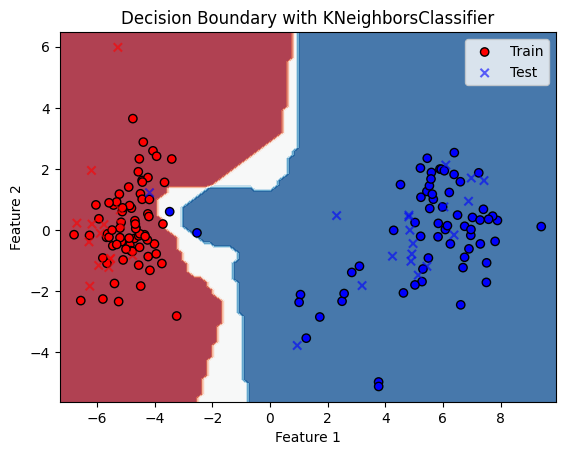
\includegraphics[width=\textwidth]{images/knn_graph.png}
    \end{figure}

	\begin{figure}[H]
        \centering
        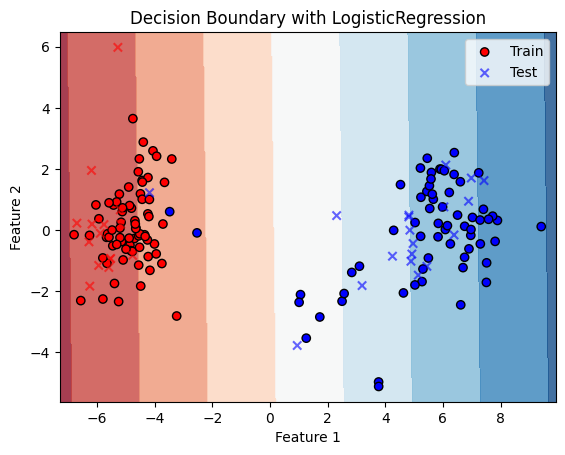
\includegraphics[width=\textwidth]{images/LR graph.png}
    \end{figure}
	\begin{figure}[H]
        \centering
        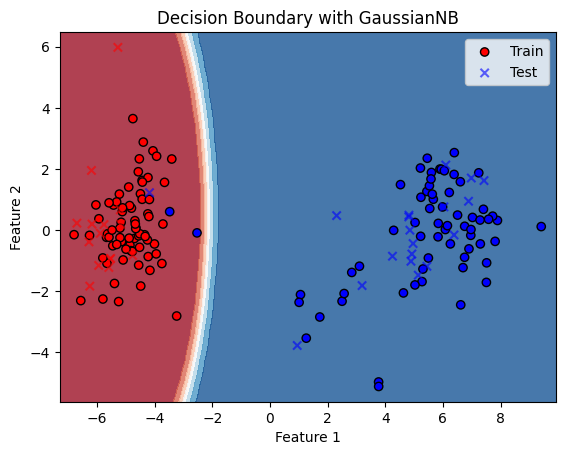
\includegraphics[width=\textwidth]{images/nb_graph.png}
    \end{figure}
	
\end{enumerate}

\printbibliography
\end{document}
